\section{Data Acquisition}
\label{section:data}



\textbf{Define region, location, object.....}
\emph{Objects} are any physical entity. For example, a \textit{tree, building, lake, bridge, gate} or \textit{sign} could be objects. \textit{Objects} can also have attributes that provide amplifying information about the object, including things like \textit{color, material, size, species etc.}. 

\emph{Locations} are physical entities that \textit{do} something. They are the meaningful grouping of objects determined by ownership, proximity or utility. They have some purpose other than being an object. They could be a \textit{business, attraction, property etc.}. 



To maximize dataset coverage, and demonstrate the flexibility of \emph{GESTALT} we support three methods of adding objects. 
In decreasing order of reliability, users can add objects by ingesting KML Files that they have manually annotated, crowd-source tags by querying the Open Street Maps API and automatically through the processing of geolocated photos. 
Each object is assigned a confidence score on ingest, reflecting the certainty that the object tagged at that location is actually the object at that location. 
Hand-labeled objects are defaulted to a confidence score of $1$, OSM objects to $0.75$ and objects labeled by the object detector are based on the confidence score reported by the object detection model. 

\subsection{Ground Truth Hand Labeled Tags}
The first method we use to obtain object tags is by hand labeling them. 
Hand labeled objects are those that have been manually annotated by a trustworthy source, they are assumed to be correctly labeled and correctly positioned. 
The reason we accept hand-labeled objects is to allow for prior manual annotation work to be folded into \emph{GESTALT}'s database. 

For benchmarking purposes we curated the Swan Valley Wineries dataset containing ground truth object tags and their associated locations stored in Keyhole Markup Language~\footnote{\href{https://developers.google.com/kml/documentation/kml_tut}{https://developers.google.com/kml/documentation/kml_tut}} (KML).
The object tagging was conducted manually by a single annotator, combining on-the-ground knowledge with manual inspection of satellite imagery, street-view imagery and publicly available photos of the area. 
The objects tagged are representative, not exhaustive. 
The object tags are aligned with ... 
The tagging was conducted using \textit{Google Earth Professional version 7.3\footnote{\href{https://www.google.com/earth/about/versions/}{https://www.google.com/earth/about/versions/}}}
Attributes of the objects (e.g. color, size, material) are recorded in the comments field as key:value pairs.
Each object from the hand-labeled dataset is assigned a confidence score of 1.0, since it is manually identified and tagged.

%NSCH: is the below sentence about the labeling or the module that aggregates all the sources? Or no longer relevant?
%The KML parser leverages the \textit{fastKML}\footnote{\href{https://pypi.org/project/fastkml/}{Fast KML PyPI Repo}} and ingests a KML file divided by region (where each region is a bounding box covering an arbitrary number of locations). 
%The KML Parser extracts the objects into dictionaries organized by location before exporting the files as JSON for future analysis. 

\begin{figure*}[ht]
\label{fig:loc}        
\includegraphics[width=0.5\textwidth]{papers/figures/loc_labels_plot.png}
\centering
\caption[width=\textwidth]{............}
\end{figure*}


\begin{figure*}[ht]
\label{fig:loc-obj}        
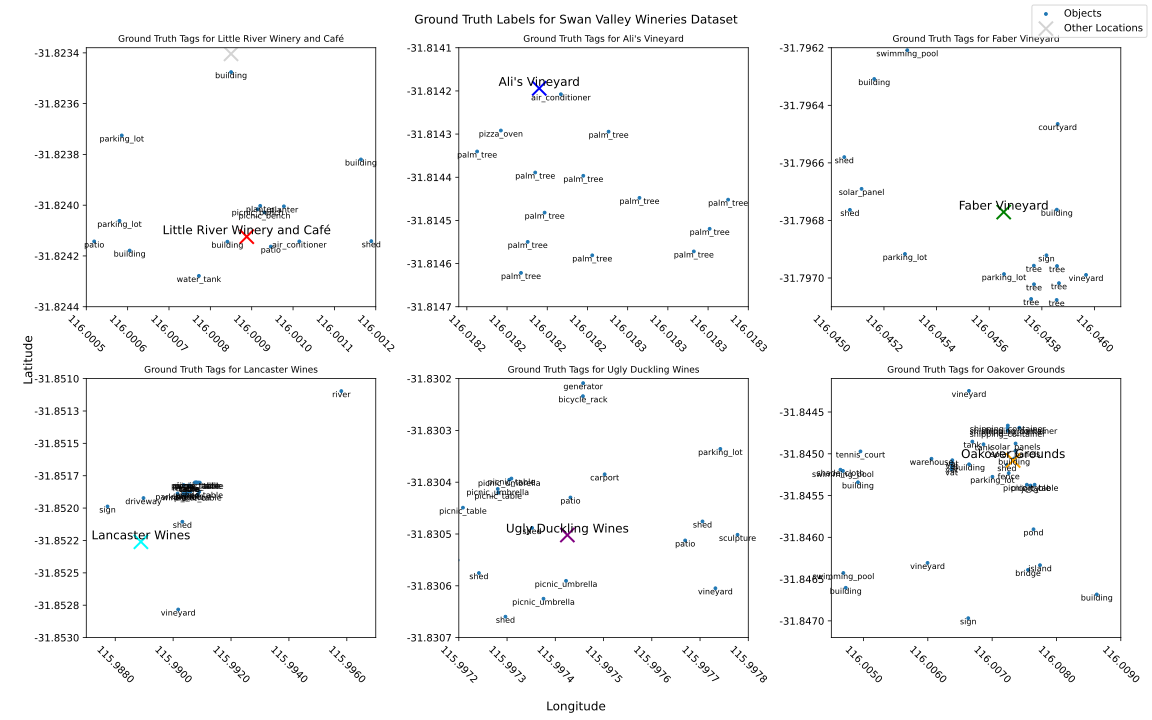
\includegraphics[width=\textwidth]{papers/figures/loc_obj_labels_plot.png}
\centering
\caption[width=\textwidth]{............}
\end{figure*}


\subsection{OSM Object Tags}
The second method involves leveraging existing OSM object tags.
While businesses, attractions and other 'locations' are commonly annotated by the OSM community, objects are more sparsely tagged, since few people have the patience to manually label apparently inconsequential things like trees, statues, fountains and telephone poles. 
\emph{GESTALT} ingests what object tags do exist in OSM through 
............describe the process here (API?)................
Each object ingested from OSM is assigned a confidence score of 1.0, since these tags are maintained by the open-source community and are subject to some degree of review and .......explain why we have some confidence in them.............


\subsection{Noisy Image-based Tags}
The third, and most important method by which \emph{GESTALT} ingests objects, is through automatic object detection.
Given a set of images and their associated geo data, ...........what is it actually called?........... the Object Detection module uses YOLO~\footnote{\href{https://github.com/ultralytics/ultralytics}{YOLO}} to identify objects in each image. Those objects are then tagged with the geolocation of the image, and stored...........how?........... For our experiments, we pull ..............how many?............ images over ............timeframe.......... and use pre-trained YOLO v.8 to detect objects from 80 classes (based on the COCO dataset.........footnote........). Each object identified is assigned a probability score ...........how does YOLO get that????..........



%%%%%%%%%%%%%%%NSCH clean up, incorporate, and delete the text below this point
The data acquisition component of \textit{GESTALT} begins with a visual encoding of the world. 
The visual encoding is primarily remote sensing imagery providing a top-down view of the earth's surface, but it also includes street-view imagery and other photographs. 
The system collects two types of information from this imagery, \textit{locations} and \textit{objects}. 
These two information types are discussed in section \ref{section:datasets}. 
Briefly recapping, objects are any physical thing in the world, and locations are the specific uses of a place that usually contains collections of objects. 

The vision for a mature data collection system enables the autonomous collection of location and object data. 
The collection system will source location data from open-access systems like OSM and relies on crowd-sourced information. 
Businesses, attractions and other higher-level 'locations' are likely to be annotated by the open-source community or business owners themselves. 
Objects, the core of \textit{GESTALT}, are much less likely to be annotated. Few people have the patience to manually tag the geolocation of apparently inconsequential things like trees, statues, fountains and telegraph poles. 
An automated solution aims to leverage publicly available remote sensing imagery data (Bing Maps Satellite data, for example) and public streetview and photo contributions to automatically identify objects, geo-locate them and add those tags to a database. 

The design for this subsystem breaks maps into small geographically-bounded chunks (approximately the size of a 'location'). 
It will use remote-sensing imagery to create a grid of objects / not-object. It will retrieve ground-level imagery within and adjacent to that box.
The first challenge is classifying an image as 'indoors' (where no objects will be visible from RSI and the closest building will 'own' it) or 'outdoors', where objects can map to the RSI. Numerous approaches exist to the indoor/outdoor scene classification \cite{Tong2017}. 
Each object in an outdoor photo's distance from the camera geolocation will be estimated using a myriad of depth estimation techniques \cite{Ming2021,Liu2020}. 
Where multiple images cover the same area from different perspectives, the composite of these images will be used to estimate the positions of objects, as has been shown in prior work like IM2GPS from Carnegie Mellon University \cite{Hays2008} and numerous other efforts over internet-available images \cite{Snavely2011}. 
As discussed in the following sub-section, some errors are permissible here and being 'close enough' is good enough as a starting point for the following systems. 





The data extraction, cleaning and loading are implemented in Python in two parts, the \textit{KML parser} for object extraction and the \textit{Open Street Maps} query interface for location retrieval. 
The KML parser leverages the \textit{fastKML}\footnote{\href{https://pypi.org/project/fastkml/}{Fast KML PyPI Repo}} and ingests a KML file divided by region (where each region is a bounding box covering an arbitrary number of locations). 
Within each region (for this test dataset), each location is separated, with its objects stored as its children. 
Attributes of the objects (e.g. colour, size, material) are recorded in the comments field as key:value pairs.
The KML Parser extracts the objects into dictionaries organised by location before exporting the files as JSON for future analysis. 

The OSM query interface leverages the \textit{OSMPythonTools}\footnote{\href{https://pypi.org/project/OSMPythonTools/}{OSMPythonTools PyPI Repo}}. It passes a bounding box to the OSM Overpass-Turbo API\footnote{\href{https://overpass-turbo.eu/}{Overpass-Turbo API}} and requests the relevant location nodes in the area. 
The results are arranged into a dictionary and exported as JSON for further analysis.








\emph{GESTALT} requires a list of all \textit{objects} with their coordinates and a list of all \textit{locations} with their coordinates. These objects and locations can be obtained in a variety of ways, which we briefly outline below. 

\subsubsection{Objects}
\paragraph{Open Street Maps (OSM)}
\textit{Open Street Maps (OSM)} is a knowledge collective that contains open-source Geodata~\cite{Haklay2008}, which can be easily extended via their online editing interface.
%NSCH tighten this up
The primary concern with OSM is the accuracy and validity of crowd-sourced data \cite{VargasMunoz2020}. However, a combination of human review and an application of machine learning for detecting anomalous behavior in OSM edits \cite{Mooney2017} goes a long way toward addressing these concerns. 

OSM records objects' coordinates as a mixture of point coordinates and bounding polygons. 
OSM has a defined and curated ontology that defines the labeling scheme, maximizing interoperability. 
The OSM objects are crowd-sourced and of varying granularity and completeness. Incompleteness is part of the initial scope of OSM, with the founder noting that it's typically only what people want to add that gets added \cite{Haklay2008}.
In general, the completeness of OSM is unassured, so scaling \textit{GESTALT} beyond the trivial requires an automated method for object detection and resolution. 
Because of the lack of completeness and to enable evaluation with ground-truth labels, the Author used Google Earth to annotate objects present at six wineries within the Swan Valley Region of Western Australia. The wineries are separated in space and a semi-rural environment. The tags consist of an object name, its latitude \& longitude, and any descriptive markings written as key:value pairs. The objects are stored by their ground truth parent location in a KML file. Additional dataset creation for the small New South Wales town of Buladelah aims to fill a 'suburban' setting and of the Darby St Restaurant Strip in Newcastle, New South Wales, for an 'urban' environment. 

\subsubsection{Locations}
%NSCH tighten this up
Google Maps\footnote{\href{https://www.google.com/maps/about/}{Google Maps}} maintains \textit{locations} as coordinate points with associated metadata. The locations are generally current and complete. 
Google Maps does not support bounding polygons at the location level; it appears to extend to as granular as ZIP Codes or suburb boundaries and no further. 
OSM Supports locations, but is less complete than Google Maps (at least for Australian Wine Regions.)
In general, for \textit{GESTALT} to function optimally, the input locations should be the union of Google Maps and OSM. However, given the limitations of Google Maps API usage, a dataset was manually curated in OSM using publicly available information and the Author's world knowledge. 
Creating the Swan Valley Winery dataset for this project has the benefit of yielding 31 additional nodes and associated metadata for the OSM project. 
